\documentclass[border=10pt]{standalone}
\usepackage[svgnames]{xcolor}
\usepackage{amsmath}
\usepackage{pgfplots}
\pgfplotsset{compat=newest}
\usepackage[sfdefault]{FiraSans}
\usepackage{FiraMono}
\renewcommand*\familydefault{\sfdefault}
\begin{document}
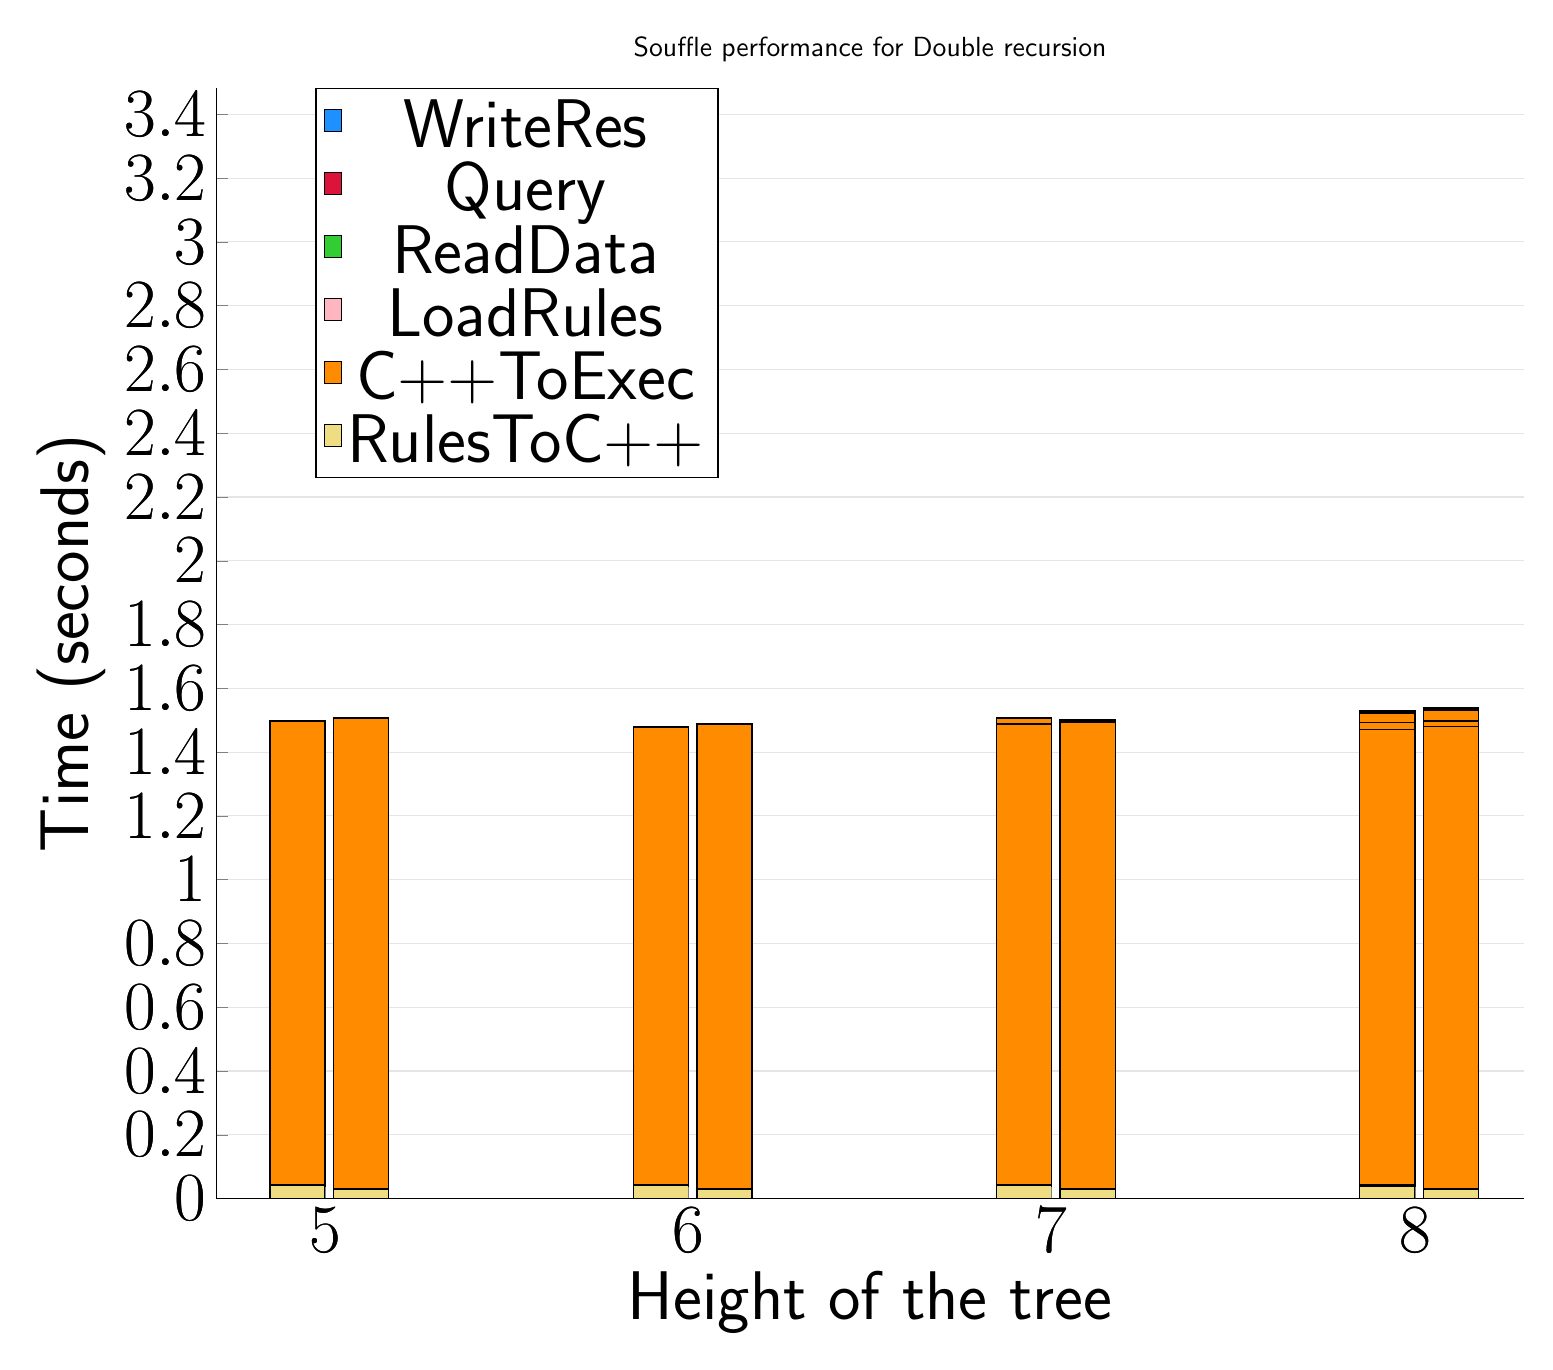
\begin{tikzpicture}
	\begin{axis}[
			ybar stacked,
			title={Souffle performance for Double recursion},
			bar shift=-10pt,
			width=1.5\textwidth,
			bar width=0.7cm,
			ymajorgrids, tick align=inside,
			major grid style={draw=gray!20},
			xtick=data,
			ymin=0, ymax=3.4829999685287474,
			axis x line*=bottom,
			axis y line*=left,
			enlarge x limits=0.1,
			legend style={
					at={(0.23, 1)},
					anchor=north,
					legend columns=1,
					font=\Huge,
				},
			ylabel={Time (seconds)},
			xlabel={Height of the tree},
			label style={font=\Huge},
			tick label style={font=\Huge},
		]
		\addlegendimage{fill=DodgerBlue, draw=black, line width=0.2pt}
		\addlegendentry{WriteRes}
		\addlegendimage{fill=Crimson, draw=black, line width=0.2pt}
		\addlegendentry{Query}
		\addlegendimage{fill=LimeGreen, draw=black, line width=0.2pt}
		\addlegendentry{ReadData}
		\addlegendimage{fill=LightPink, draw=black, line width=0.2pt}
		\addlegendentry{LoadRules}
		\addlegendimage{fill=DarkOrange, draw=black, line width=0.2pt}
		\addlegendentry{C++ToExec}
		\addlegendimage{fill=LightGoldenrod, draw=black, line width=0.2pt}
		\addlegendentry{RulesToC++}
		\addplot +[fill=LightGoldenrod, draw=black, line width=0.5pt] coordinates {
				(5, 0.04200000762939453)
				(6, 0.042999982833862305)
				(7, 0.040999984741210936)
				(7, 0.04200000762939453)
				(7, 0.042999982833862305)
				(8, 0.039999985694885255)
				(8, 0.04200000762939453)
				(8, 0.04000005722045898)
			};
		\addplot +[fill=DarkOrange, draw=black, line width=0.5pt] coordinates {
				(5, 1.455999994277954)
				(6, 1.4349999904632569)
				(7, 1.447000002861023)
				(7, 1.4469999551773072)
				(7, 1.462000036239624)
				(8, 1.4829999685287476)
				(8, 1.4509999990463256)
				(8, 1.4309999465942382)
			};
		\addplot +[fill=LightPink, draw=black, line width=0.5pt] coordinates {
				(5, 0.00011953340000000001)
				(6, 8.85168e-05)
				(7, 9.985409999999999e-05)
				(7, 0.0001007961)
				(7, 6.882910000000001e-05)
				(8, 8.505000000000001e-05)
				(8, 0.00011194599999999999)
				(8, 0.00011135)
			};
		\addplot +[fill=LimeGreen, draw=black, line width=0.5pt] coordinates {
				(5, 0.0002915875)
				(6, 0.00040420429999999996)
				(7, 0.0005481708999999999)
				(7, 0.000537196)
				(7, 0.0004942919)
				(8, 0.00077165)
				(8, 0.0008200083)
				(8, 0.0008308082)
			};
		\addplot +[fill=Crimson, draw=black, line width=0.5pt] coordinates {
				(5, 0.0002667209)
				(6, 0.0008389958999999999)
				(7, 0.002230479)
				(7, 0.002206612)
				(7, 0.0019910080000000003)
				(8, 0.005410509)
				(8, 0.005709113000000001)
				(8, 0.005893685)
			};
		\addplot +[fill=DodgerBlue, draw=black, line width=0.5pt] coordinates {
				(5, 0.0004124084)
				(6, 0.0006677789)
				(7, 0.0006686341)
				(7, 0.0005815082)
				(7, 0.0007282037)
				(8, 0.0008849248000000001)
				(8, 0.0010179746)
				(8, 0.0009156250000000001)
			};
	\end{axis}
	\begin{axis}[
			ybar stacked,
			bar shift=13pt,
			width=1.5\textwidth,
			bar width=0.7cm,
			ymajorgrids, tick align=inside,
			major grid style={draw=none},
			xtick=data,
			ymin=0, ymax=3.4829999685287474,
			axis x line*=none,
			axis y line*=none,
			enlarge x limits=0.1,
			label style={font=\Huge},
			tick label style={font=\Huge},
		]
		\addplot +[fill=LightGoldenrod, draw=black, line width=0.5pt] coordinates {
				(5, 0.030000000000000006)
				(6, 0.030000000000000006)
				(7, 0.031000000000000007)
				(7, 0.030000000000000006)
				(7, 0.030000000000000006)
				(8, 0.030000000000000006)
				(8, 0.031000000000000007)
				(8, 0.030000000000000006)
			};
		\addplot +[fill=DarkOrange, draw=black, line width=0.5pt] coordinates {
				(5, 1.4760000000000002)
				(6, 1.4579999999999997)
				(7, 1.4659999999999997)
				(7, 1.465)
				(7, 1.4620000000000002)
				(8, 1.5020000000000002)
				(8, 1.467)
				(8, 1.4509999999999996)
			};
		\addplot +[fill=LightPink, draw=black, line width=0.5pt] coordinates {
				(5, 0.00011860000000000002)
				(6, 8.8e-05)
				(7, 9.92e-05)
				(7, 9.96e-05)
				(7, 6.82e-05)
				(8, 7.439999999999999e-05)
				(8, 0.0001104)
				(8, 0.0001098)
			};
		\addplot +[fill=LimeGreen, draw=black, line width=0.5pt] coordinates {
				(5, 0.0002906)
				(6, 0.00040349999999999994)
				(7, 0.0005455)
				(7, 0.0005363)
				(7, 0.0004936)
				(8, 0.0007706000000000001)
				(8, 0.0008191)
				(8, 0.0008298000000000001)
			};
		\addplot +[fill=Crimson, draw=black, line width=0.5pt] coordinates {
				(5, 0.0002662)
				(6, 0.0008383999999999999)
				(7, 0.0022268)
				(7, 0.0022058999999999994)
				(7, 0.0019904)
				(8, 0.005409000000000001)
				(8, 0.0057082)
				(8, 0.0058922)
			};
		\addplot +[fill=DodgerBlue, draw=black, line width=0.5pt] coordinates {
				(5, 0.00026849999999999997)
				(6, 0.0003728)
				(7, 0.0005154000000000001)
				(7, 0.0005147999999999999)
				(7, 0.0004741)
				(8, 0.0008629999999999998)
				(8, 0.0009075)
				(8, 0.0009140999999999999)
			};
	\end{axis}
\end{tikzpicture}

\end{document}
